\documentclass{article}

\usepackage{amsmath, amsthm, amssymb, amsfonts}
\usepackage{thmtools}
\usepackage{graphicx}
\usepackage{setspace}
\usepackage{geometry}
\usepackage{float}
\usepackage[hidelinks]{hyperref}
\usepackage[utf8]{inputenc}
\usepackage[spanish]{babel}
\usepackage{framed}
\usepackage[dvipsnames]{xcolor}
\usepackage{tcolorbox}
\usepackage{tikz}
\usepackage{caption}
\usepackage{longtable}
\usepackage{pdflscape}
\usepackage{svg}
\usepackage{subcaption}
\usepackage{caption}
\usepackage{multirow}
\usepackage{array}
\usepackage{listings}

\colorlet{LightGray}{White!90!Periwinkle}
\colorlet{LightOrange}{Orange!15}
\colorlet{LightGreen}{Green!15}



\newcommand{\HRule}[1]{\rule{\linewidth}{#1}}

\declaretheoremstyle[name=Theorem,]{thmsty}
\declaretheorem[style=thmsty,numberwithin=section]{theorem}
\tcolorboxenvironment{theorem}{colback=LightGray}

\declaretheoremstyle[name=Proposition,]{prosty}
\declaretheorem[style=prosty,numberlike=theorem]{proposition}
\tcolorboxenvironment{proposition}{colback=LightOrange}

\declaretheoremstyle[name=Principle,]{prcpsty}
\declaretheorem[style=prcpsty,numberlike=theorem]{principle}
\tcolorboxenvironment{principle}{colback=LightGreen}

\newcolumntype{L}[1]{>{\raggedleft\let\newline\\\arraybackslash\hspace{0pt}}m{#1}}
\newcolumntype{C}[1]{>{\centering\let\newline\\\arraybackslash\hspace{0pt}}m{#1}}
\newcolumntype{R}[1]{>{\raggedright\let\newline\\\arraybackslash\hspace{0pt}}m{#1}}

\setstretch{1.2}
\geometry{
    textheight=9in,
    textwidth=5.5in,
    top=1in,
    headheight=12pt,
    headsep=25pt,
    footskip=30pt
}

\lstdefinestyle{bashstyle}{
    language=bash,
    basicstyle=\ttfamily,
    backgroundcolor=\color{gray!10},
    keywordstyle=\color{blue},
    commentstyle=\color{green!40!black},
    stringstyle=\color{red},
    showstringspaces=false,
    numbers=left,
    numberstyle=\tiny\color{gray},
    breaklines=true,
    breakatwhitespace=true,
    frame=tb,
    rulecolor=\color{black!70},
    framerule=0.5pt,
    tabsize=4,
    captionpos=b
}

\lstdefinestyle{javastyle}{
    language=Java,
    basicstyle=\ttfamily,
    backgroundcolor=\color{gray!10},
    keywordstyle=\color{blue},
    commentstyle=\color{green!40!black},
    stringstyle=\color{red},
    showstringspaces=false,
    numbers=left,
    numberstyle=\tiny\color{gray},
    breaklines=true,
    breakatwhitespace=true,
    frame=tb,
    rulecolor=\color{black!70},
    framerule=0.5pt,
    tabsize=4,
    captionpos=b
  }

 \lstdefinestyle{pythonstyle}{
    language=Python,
    basicstyle=\ttfamily\small,
    keywordstyle=\bfseries\color{blue},
    commentstyle=\itshape\color{gray},
    stringstyle=\color{green},
    numberstyle=\tiny\color{gray},
    identifierstyle=\color{black},
    breaklines=true,
    showstringspaces=false,
    numbers=left,
    numbersep=5pt,
    frame=single,
    tabsize=4,
    captionpos=b,
    morekeywords={self}  % Add keywords here
}

% ------------------------------------------------------------------------------

\begin{document}

\title{ \normalsize \textsc{}
	\\ [2.0cm]
	\HRule{1.5pt} \\
	\LARGE \textbf{\uppercase{python for data analysis}
		\HRule{2.0pt} \\ [0.6cm] \LARGE{Third Edition} \vspace*{10\baselineskip}}
}
\date{}
\author{\textbf{Alvarado Becerra Ludwig} \\
	El ingeniero más lamentable}

\maketitle
\thispagestyle{empty}
\newpage

\tableofcontents
\thispagestyle{empty}
\newpage
\setcounter{page}{1}


\section{Numpy Basics: Arrays and Vectorized Computation}

Numpy proporciona:

\begin{itemize}
  \item Operaciones basadas en arrays haciendo que todo el proceso se lleve a otro tipo de computación.
  \item Proporciona algoritmos comúnes como ordenar, único, y operaciones de conjunto.
  \item Operaciones estadísticas rápidas.
  \item Arreglos de manipuladores de datos para unir y fusionar datasets heterogéneos.
  \item Expresar condiciones lógicas como arrays en lugar de ciclos con if-elif-else.
  \item Manipulaciones de grupos (agregación, transformación, y aplicaciones de función).
\end{itemize}

Numpy da una fundación computacional para un procesamiento general de los datos. Pandas, da algunas funciones más específicas como manipulación de series de tiempo, algo que no está en Numpy.

Numpy almacena los datos en un bloque de memoria continuo, independiente de otros objetos construidos en Python. Sus arrays también utilizan mucho menos memoria que las construidas en Python.

Se va a ejecutar el siguiente código para probar esta diferencia de velocidad.

\begin{lstlisting}[style=pythonstyle]
import numpy as np

my_arr = np.arange(1_000_000)

my_list = list(range(1_000_000))
\end{lstlisting}

Ahora, multiplicando cada lista/array por dos, se obtiene el siguiente resultado:

\begin{figure}[H]
  \centering
  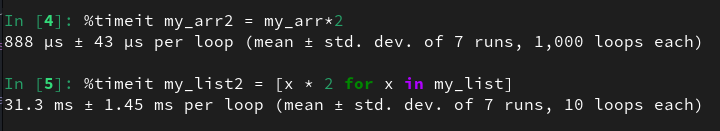
\includegraphics[width=1\textwidth]{img/Img1.png}
\end{figure}

Se obtiene una diferencia de escalas de miles a micro segundos, por lo tanto, se comprueba que las arrays en Numpy son muy eficientes.

\subsection{La ndarray: Una array multidimensional}

Las arrays permiten realizar operaciones matemáticas de bloques de datos utilizando sintaxis similar a las equivalentes entre elementos escalares.

Una ndarray es un contenedor multidimensional genérico para datos homogéneos, eso tiene que ser así, todos los elementos deben tener el mismo \textit{data type}. Todo dato tiene una \textit{shape}, una tupla que indica el tamaño de cada dimensión, y un \textit{dtype}, un objeto describiendo el \textit{data type} de la array.

\begin{lstlisting}[style=pythonstyle]
In [1]: import numpy as np

In [2]: data = np.array([[1.5, -0.1, 3], [0, -3, 6.5]])

In [3]: data
Out[3]:
array([[1.5, -0.1, 3. ],
       [0. , -3. , 6.5]])

In [4]: data.shape
Out[4]: (2, 3)

In [5]: data.dtype
Out[5]: dtype('float64')
\end{lstlisting}

Las filas son lo que le da dimensión a las arrays, por ejemplo:

\begin{lstlisting}{style=pythonstyle}
In [1]: data2 = [[1, 2, 3, 4], [5, 6, 7, 8]]

In [2]: arr2 = np.array(data2)

In [3]: arr2
Out[3]:
array([[1, 2, 3, 4],
      [5, 6, 7, 8]])

In [4]: arr2.ndim
Out[4]: 2

In [5]: arr2.shape
Out[5]: (2, 4)
\end{lstlisting}

La primera posición del \textit{shape} es la dimensionalidad, o las filas del array, mientras que la segunda posición son las columnas del array.

\subsection{Tipos de datos}

A continuación, se presentan los tipos de datos que se pueden manejar en Numpy


\begin{longtable}{|C{0.25\textwidth}|C{0.25\textwidth}|C{0.4\textwidth}|}
  \hline
  \textbf{\textit{Type}} & \textbf{Código del \textit{type}} & \textbf{Descripción} \\ \hline
  \texttt{int8, uint8} & \texttt{i1, u1} & Enteros asignados y sin asignar de 8-bits (1 byte) \\ \hline
  \texttt{int16, uint16} & \texttt{i2, u2} & Enteros asignados y sin asignar de 16-bits (2 bytes) \\ \hline
  \texttt{int32, uint32} & \texttt{i4, u4} & Enteros asignados y sin asignar de 32-bits (4 bytes) \\ \hline
  \texttt{int64, uint64} & \texttt{i8, u8} & Enteros asignados y sin asginar de 64-bits (8 bytes) \\ \hline
  \texttt{float16} & \texttt{f2} & Mitad de precisión de un punto flotante \\ \hline
  \texttt{float32} & \texttt{f4} o \texttt{f} & Punto flotante con precisión estándar individual; compatible con el flotante de C \\ \hline
  \texttt{float64} & \texttt{f9} o \texttt{d} & Punto flotante con precisión doble; compatible con el \textit{double} de C y el objeto flotante de Python. \\ \hline
\end{longtable}





\end{document}
